
\begin{table*}[ht]
\small
\centering
\scalebox{1.0}{
\begin{tabular}{lccccccc}
\toprule
 \multicolumn{1}{c}{\multirow{2}{*}{\bf Methods}} & \multicolumn{4}{c}{\bf Accuracy} & \multicolumn{3}{c}{\bf Unanswerable Questions} \\ \cmidrule(r){2-5} \cmidrule(r){6-8} & TA & TP & TI & Overall & Precision & Recall & F1 \\ \midrule 
 SP & 18.18 & 58.82 & 30.34 & 29.83 & 46.88 & 13.39 & 20.84 \\
 CoT & 67.80 & 74.51 & 49.15 & 61.67 & 42.61 & 43.75 & 43.18 \\
 MemoChat & 35.23 & 43.14 & 25.21 & 32.67 & 24.30 & 77.68 & 37.02 \\
 Memochat + CoT & 51.14 & 49.02 & 26.50 & 41.67 & 24.80 & \bf 81.25 & 38.00 \\
 Timeline + CoT & 83.33 & 78.41 & 58.55 & 71.50 & 48.51 & 58.04 & 52.84 \\
 TReMu & \bf 84.47 & \bf 81.37 & \bf 68.38 & \bf 77.67 & \bf 55.48 & 76.79 & \bf 64.42\\
\bottomrule

\end{tabular}}
\caption{\label{gpt4o_result} Experimental results of various methods based on GPT-4o. We use TA to represent Temporal Anchoring, TP for Temporal Precedence and TI for Temporal Interval.}
% \vspace{-0.3cm}
\end{table*}

\begin{table*}[ht]
\small
\centering
\scalebox{1.0}{
\begin{tabular}{lccccccc}
\toprule
 \multicolumn{1}{c}{\multirow{2}{*}{\bf Methods}} & \multicolumn{4}{c}{\bf Accuracy} & \multicolumn{3}{c}{\bf Unanswerable Questions} \\ \cmidrule(r){2-5} \cmidrule(r){6-8} & TA & TP & TI & Overall & Precision & Recall & F1 \\ \midrule 
 SP & 20.08 & 50.00 & 29.91 & 29.00 & \bf 40.00 & 26.79 & 32.08 \\
 CoT & 46.59 & \bf 62.75 & 37.18 & 45.67 & 33.96 & 48.21 & 39.86 \\
 MemoChat & 21.21 & 39.22 & 23.50 & 25.17 & 21.11 & 74.11 & 32.88 \\
 Memochat + CoT & 24.62 & 45.10 & 24.36 & 28.00 & 21.11 & 75.00 & 32.94 \\
 Timeline + CoT & 55.68 & 59.80 & 38.46 & 49.67 & 30.73 & 59.82 & 40.60 \\
 TReMu & \bf 64.02 & 46.08 & \bf 38.89 & \bf 51.17 & 29.21 & \bf92.86 & \bf 44.44\\
\bottomrule

\end{tabular}}
\caption{\label{gpt4o_mini_result} Experimental results of various methods based on GPT-4o-mini.}
\vspace{-0.5cm}
\end{table*}

\begin{table*}[ht]
\small
\centering
\scalebox{1.0}{
\begin{tabular}{lccccccc}
\toprule
 \multicolumn{1}{c}{\multirow{2}{*}{\bf Methods}} & \multicolumn{4}{c}{\bf Accuracy} & \multicolumn{3}{c}{\bf Unanswerable Questions} \\ \cmidrule(r){2-5} \cmidrule(r){6-8} & TA & TP & TI & Overall & Precision & Recall & F1 \\ \midrule 
 SP & 21.59 & 31.37 & 23.08 & 23.83 & 22.91 & 46.43 & 30.68 \\
 CoT & 23.86 & 38.24 & 22.65 & 25.83 & 20.97 & 50.00 & 29.56 \\
 MemoChat & 17.42 & 45.10 & 23.50 & 24.50 & 21.93 & 66.96 & 33.04 \\
 Memochat + CoT & 20.45 & \bf 53.92 & \bf 26.50 & 28.50 & 21.79 & 50.00 & 30.36 \\
 Timeline + CoT & 32.58 & 44.12 & 22.65 & 30.67 & 22.57 & 51.79 & 31.44 \\
 TReMu & \bf 42.42 & 37.25 & 22.22 & \bf 33.67 & \bf 23.33 & \bf 75 & \bf 35.60\\
\bottomrule

\end{tabular}}
\caption{\label{gpt35_result} Experimental results of various methods based on GPT-3.5-Turbo.}
% \vspace{-0.3cm}
\end{table*}

\section{Experiments}
% We perform extensive experiments on our constructed benchmark for multi-session dialogues, and provide detailed results in this section.

\subsection{Experimental Setup} 
\noindent \textbf{Models.}
We build our framework using various \textit{black-box} LLMs: GPT-4o\footnote{Specifically, \textit{gpt-4o-2024-05-13}.}, GPT-4o-mini\footnote{Specifically, \textit{gpt-4o-mini-2024-07-18}.}, and GPT-3.5-Turbo\footnote{Specifically, \textit{gpt-3.5-turbo-0125}.}. Particularly, for GPT-3.5-Turbo, many of LoCoMo dialogues are longer than its input length, we then follow LoCoMo \cite{maharana-etal-2024-evaluating} which earlier dialogues are omitted. 

\label{sec:models}
Particularly, we have also tried different \textit{open-source} LLMs but most of them cannot handle the long dialogue inputs from LoCoMo, for example only about 10\% of dialogues can be fed into Llama-3-70B. And even for those shorter dialogues that can be fed into Llama-3-70B, we notice that the model gets lost and fails to follow instructions, even failing to generate in the desired format. Therefore, we leave the adaptation to LLMs as future work.

\noindent\textbf{Baselines.}
Since in our setting of multi-session dialogues where the conversations exceed the input limits of LLMs, we consider the memory mechanism as a critical component of baselines in order to feed complete dialogue information. Therefore, we include the following baselines for comparison:



\begin{itemize} 
    \item \textbf{Standard Prompting (SP)}: The entire dialogue is provided along with each temporal question, with additional instructions for selecting the correct answer.

    \item \textbf{Chain-of-Thought (CoT)} \cite{wei2022chain}: Similar to SP, but with additional instructions for LLMs to solve questions step-by-step.

    \item \textbf{MemoChat} \cite{lu2023memochat}: Given that multi-turn dialogues can exceed the model's input length, and since our approach builds on memory-augmented LLM-agents, MemoChat serves as a baseline where we modify the response stage to answer temporal questions.
\end{itemize}

To better understand the effectiveness of each component in our framework, we evaluate the following variants as baselines for the ablation study:
\begin{itemize}
    \item \textbf{MemoChat + CoT}: This baseline applies CoT in the response stage to answer temporal questions step-by-step using the retrieved memory.

    \item \textbf{Timeline + CoT}: Based on the framework of memory-augmented LLM-agents, we modify the original memorization with our proposed timeline summarization and combine it with CoT as a baseline.
\end{itemize}

Comparing MemoChat + CoT and Timeline + CoT allows us to assess the impact of replacing the standard memory mechanism in LLM agents with our time-aware memorization. Additionally, comparing Timeline + CoT with TReMu highlights the effect of replacing CoT with our neuro-symbolic reasoning approach.

\noindent\textbf{Evaluation Metrics.}
We primarily use \textbf{accuracy} to assess the overall performance of temporal reasoning. In addition, for unanswerable questions, we calculate \textbf{precision}, \textbf{recall}, and the \textbf{F1} score to specifically measure performance on this subset of questions. Specifically, precision is computed as the accuracy of questions the model predicts as "unanswerable," while recall is determined by the accuracy of questions where the ground truth answer is "unanswerable."

\subsection{Experimental Results} 
The results are shown in Tables \ref{gpt4o_result}, \ref{gpt4o_mini_result}, and \ref{gpt35_result} for GPT-4o, GPT-4o-mini, and GPT-3.5-Turbo, respectively. On the recent TRAM benchmark \cite{wang-zhao-2024-tram}, existing LLMs demonstrate strong performance with direct prompting. For instance, GPT-4 achieves an accuracy of 82 using CoT, while GPT-3.5 attains 71.40. In contrast, our benchmark is significantly more challenging. GPT-4o achieves only 61.67 with CoT and 29.83 with SP, whereas GPT-3.5 performs even worse, scoring 25.83 with CoT and 23.83 with SP. These performance gaps likely stem from the complexity of multi-session dialogues and their temporal dependencies, which are not explicitly addressed in previous benchmarks.

Our framework outperforms all baseline methods across all three LLMs in terms of both accuracy and F1 scores, with a notable increase in accuracy from 29.83 with SP to 77.67 with our framework using GPT-4o. This demonstrates the effectiveness of our approach in enhancing temporal reasoning for multi-session dialogues. However, incorporating a memory mechanism performs worse than CoT for GPT-4o and GPT-4o-mini. This may be because these models have sufficient input lengths to process LoCoMo dialogues, enabling them to identify relevant temporal information without additional memory augmentation. In contrast, for GPT-3.5, which has a shorter input limit, the memory mechanism generally improves performance by allowing the model to retrieve information from memory rather than truncated dialogues. 

% Additionally, we observe that GPT-4o-mini exhibits weaker time-aware memorization, occasionally failing to infer that events occurred at different time steps. Consequently, the agent struggles to retrieve useful memory for answering questions, leading it to select "unanswerable" options more frequently. This trend is reflected in its high recall for unanswerable questions in Table \ref{gpt4o_mini_result}. Notably, as shown in the left part of Table 4, GPT-4o-mini achieves higher accuracy for answerable questions compared to baselines. This suggests that when memory is correctly retrieved, the agent is more likely to select the correct answer. These findings highlight the importance of designing an effective memory mechanism to facilitate accurate retrieval of relevant information.

Furthermore, we find that incorporating CoT generally improves performance, aligning with previous findings \cite{wang-zhao-2024-tram,xiong-etal-2024-large}. In particular, CoT encourages models to search for relevant information within dialogues. However, due to the dialogues’ length, the models sometimes generate responses like "I cannot find the mention of ...," which hinders their temporal reasoning capabilities. This further underscores the necessity of a memory mechanism to support long dialogue settings.

\begin{figure}  
\centering
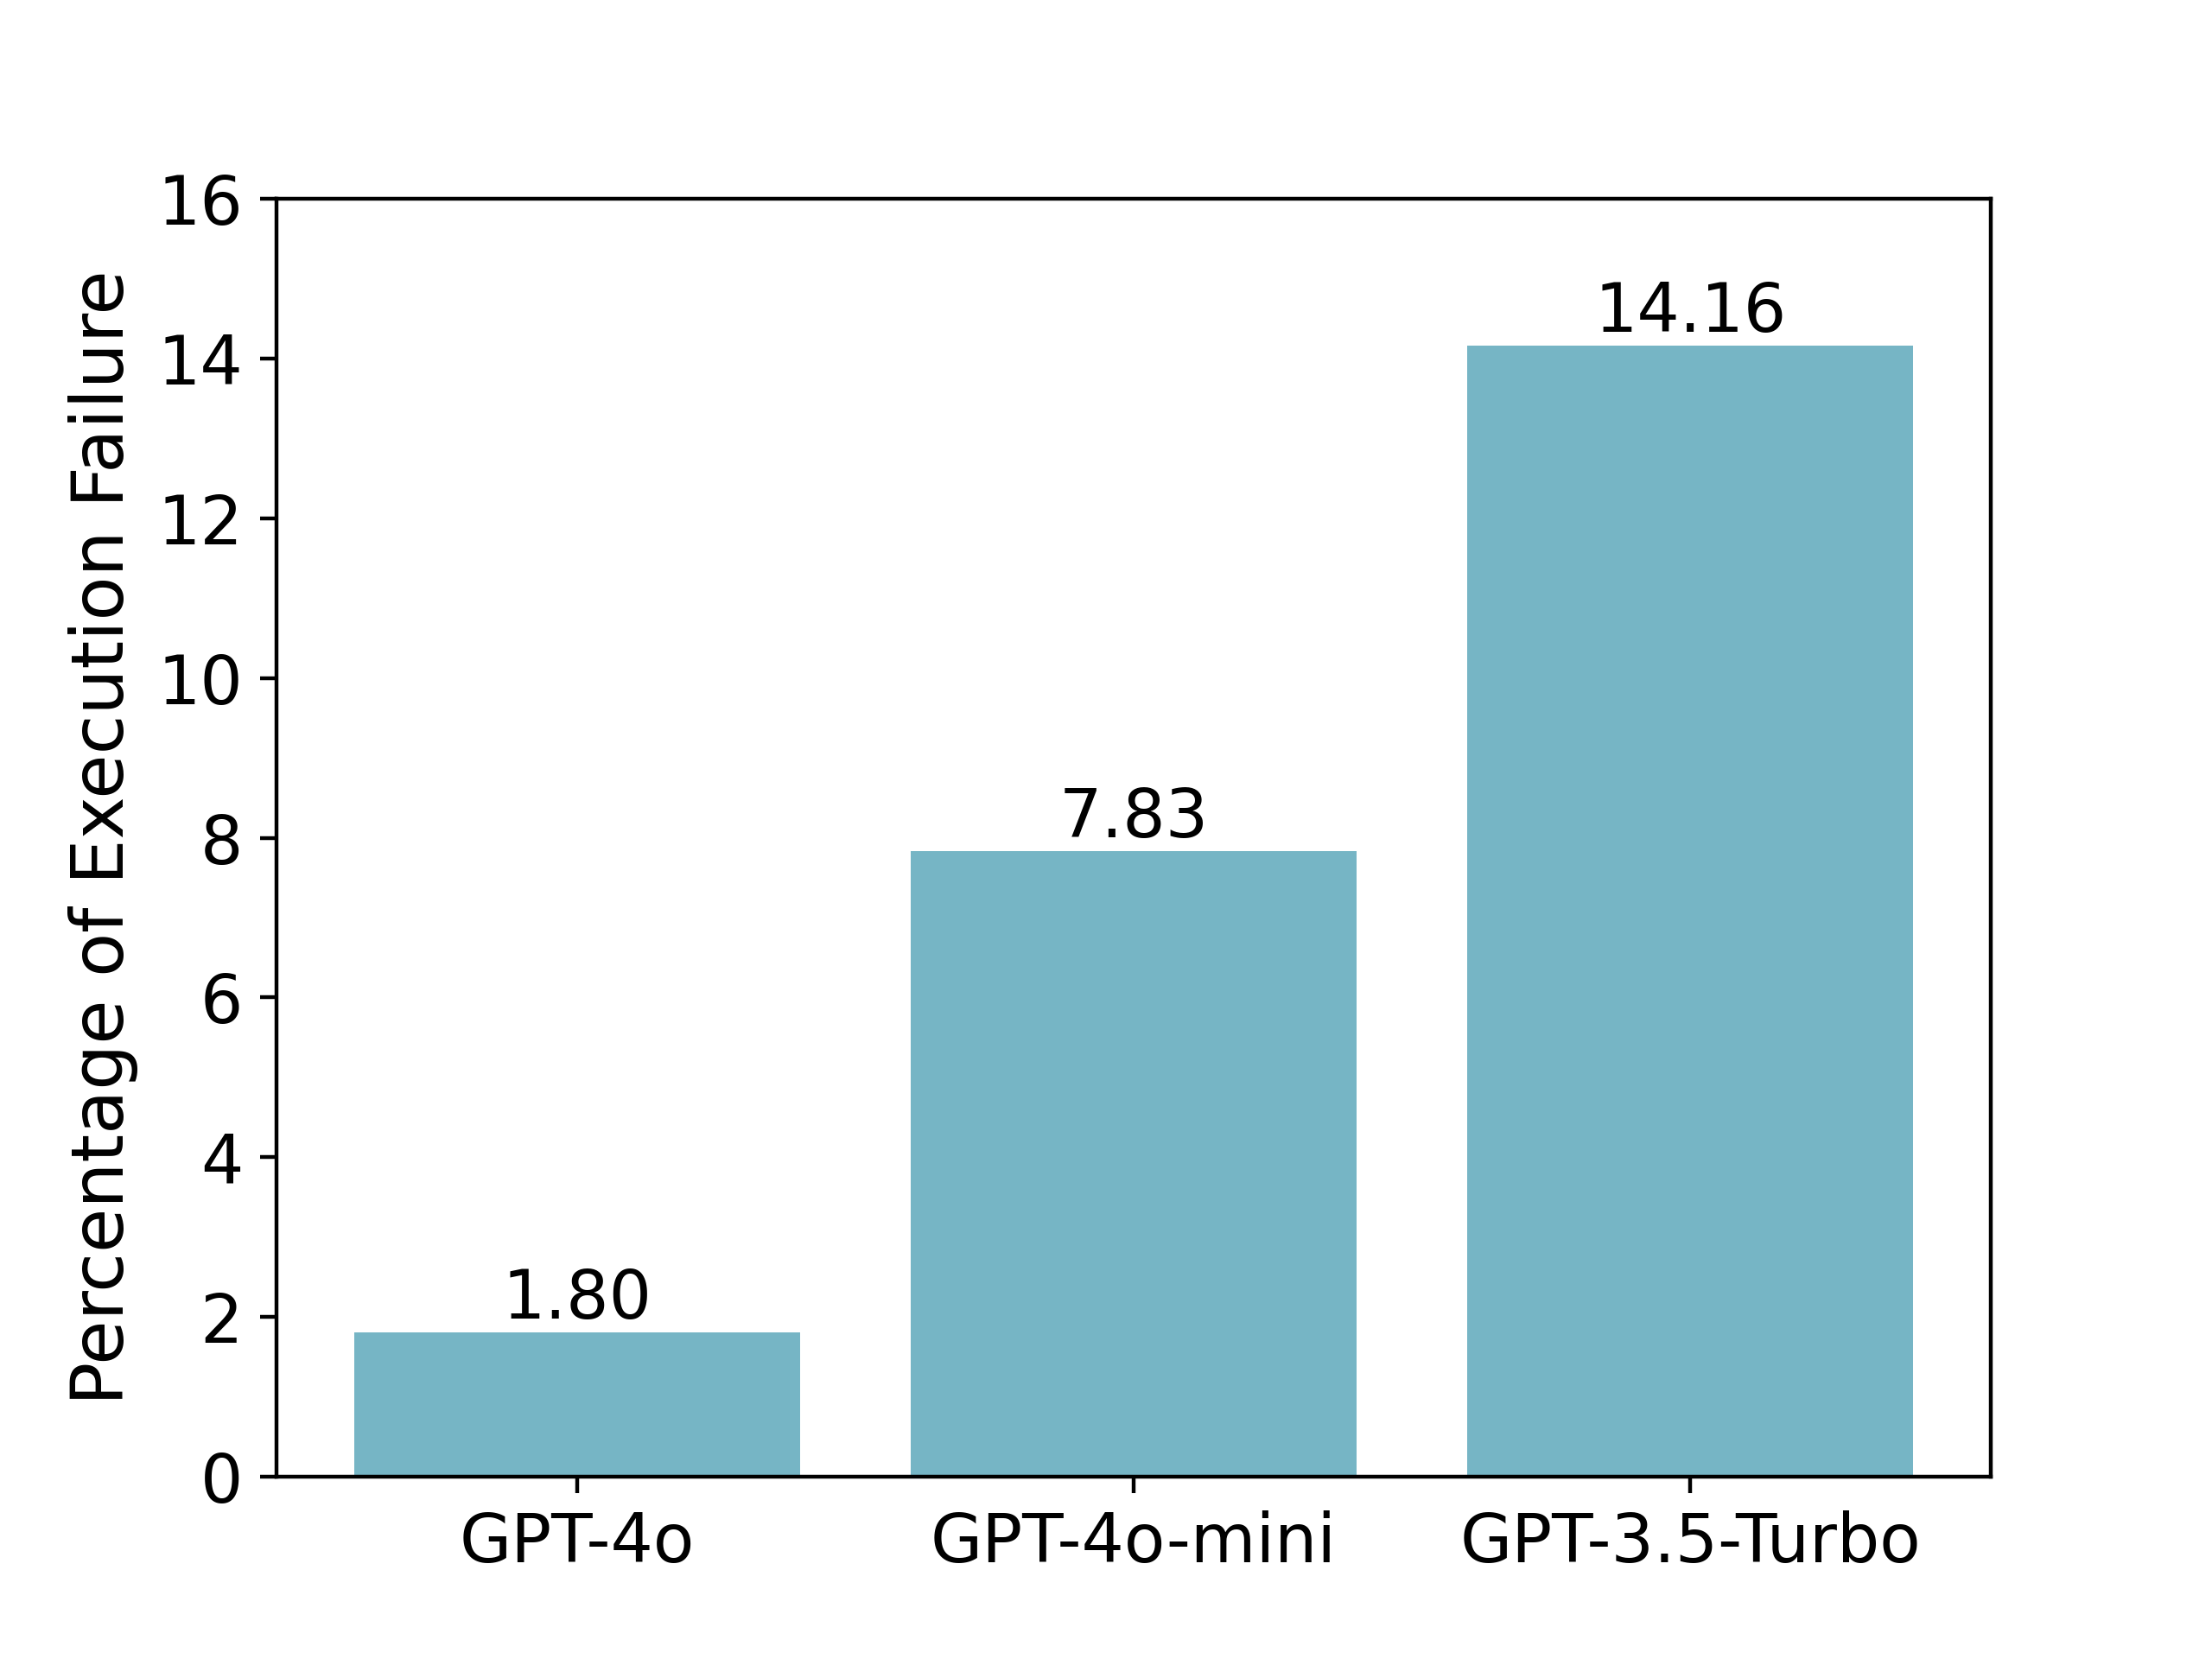
\includegraphics[width=0.85\linewidth]{figures/failure.png}
    \caption{The percentage of execution failures.} 
    \label{fig:failure}
% \vspace{-0.6cm}
\end{figure}

\begin{figure*}[t]
    \centering
    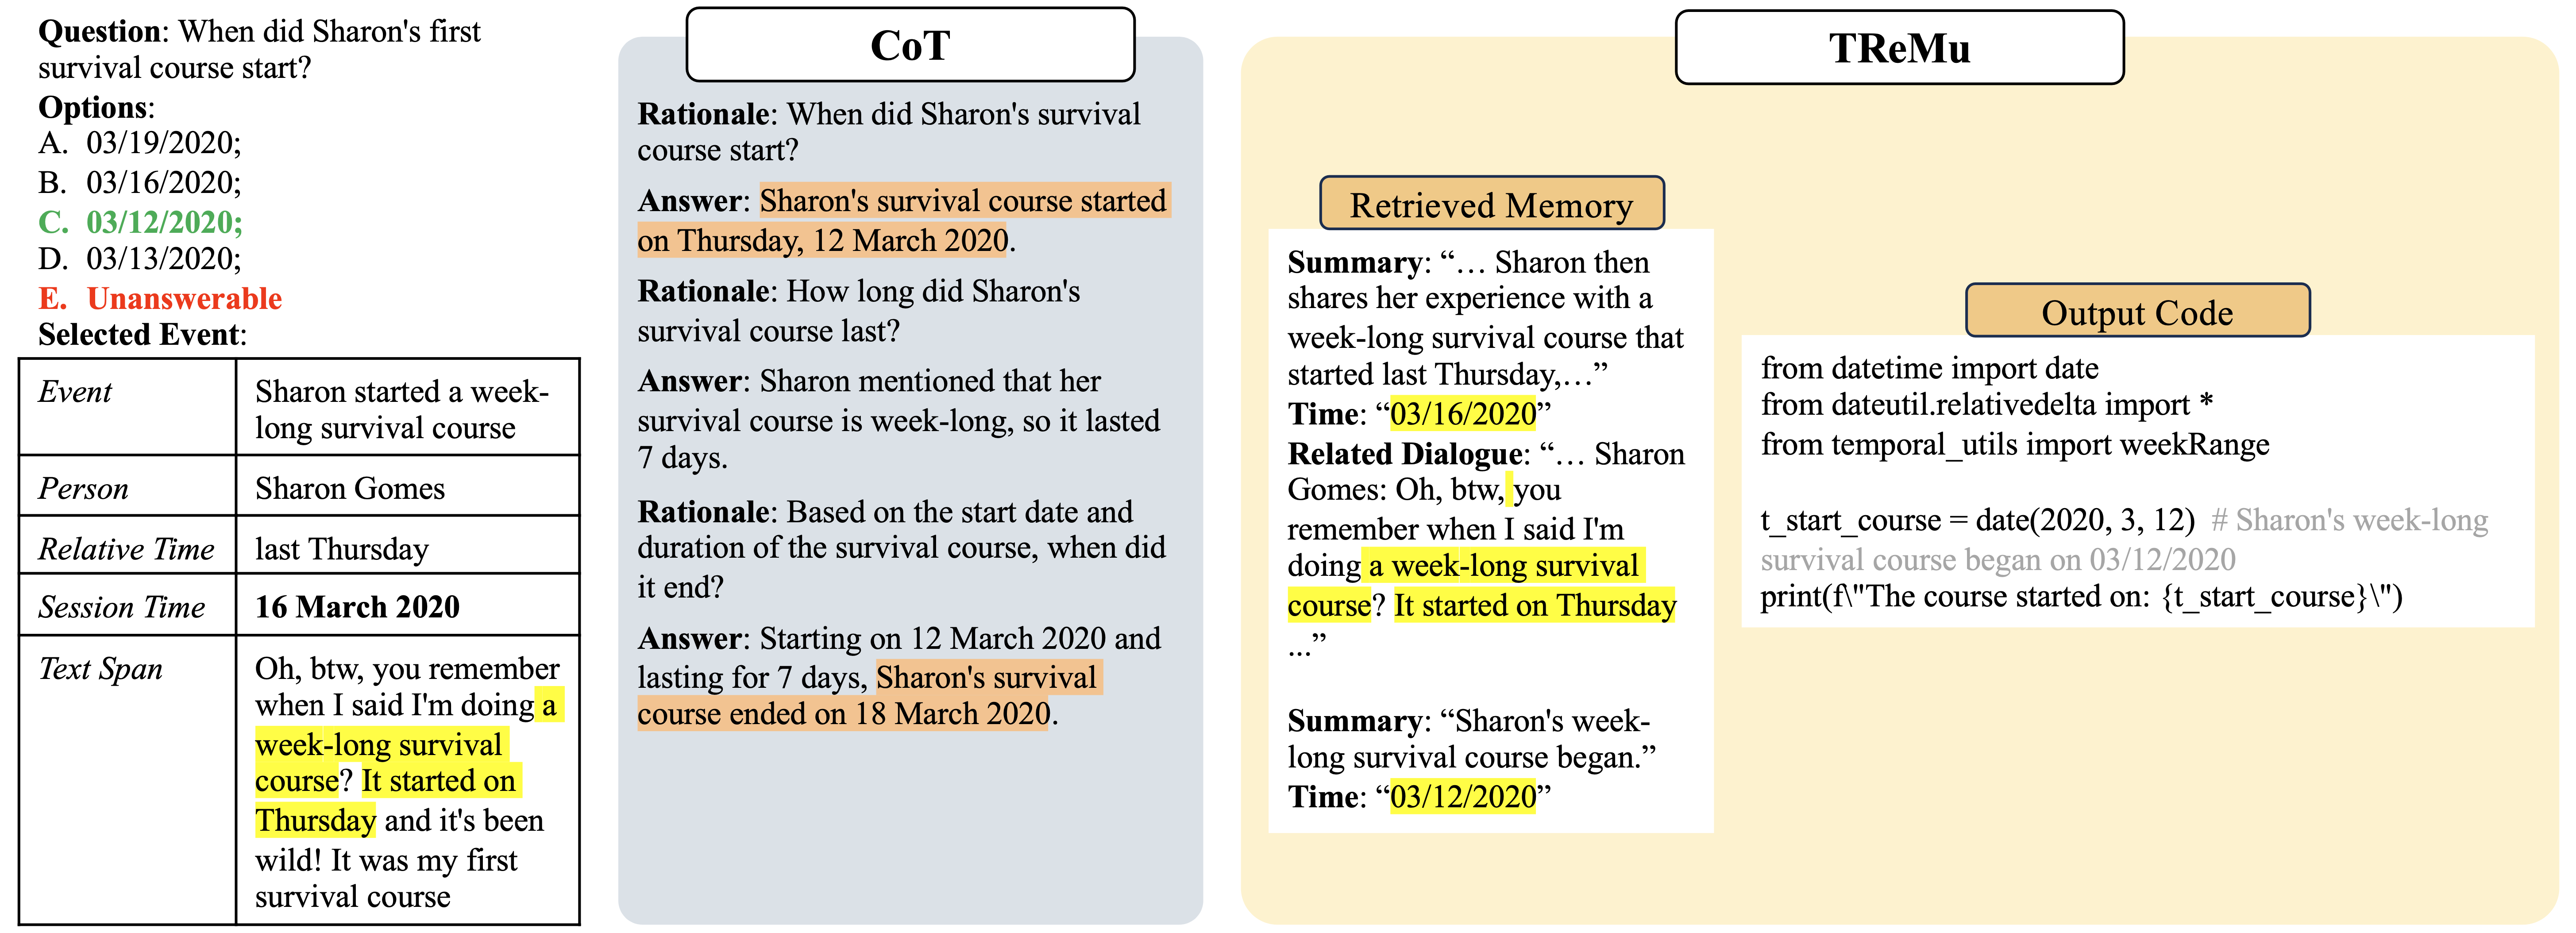
\includegraphics[width=\linewidth]{figures/case_1.png}
    \caption{The first case study comparing CoT and our proposed framework, where CoT results in the wrong answer "E" but our approach selects the correct option "C". We highlight the key information in colors.}
    \label{fig:case_1}
% \vspace{-0.5cm}
\end{figure*}

\begin{figure*}[t]
    \centering
    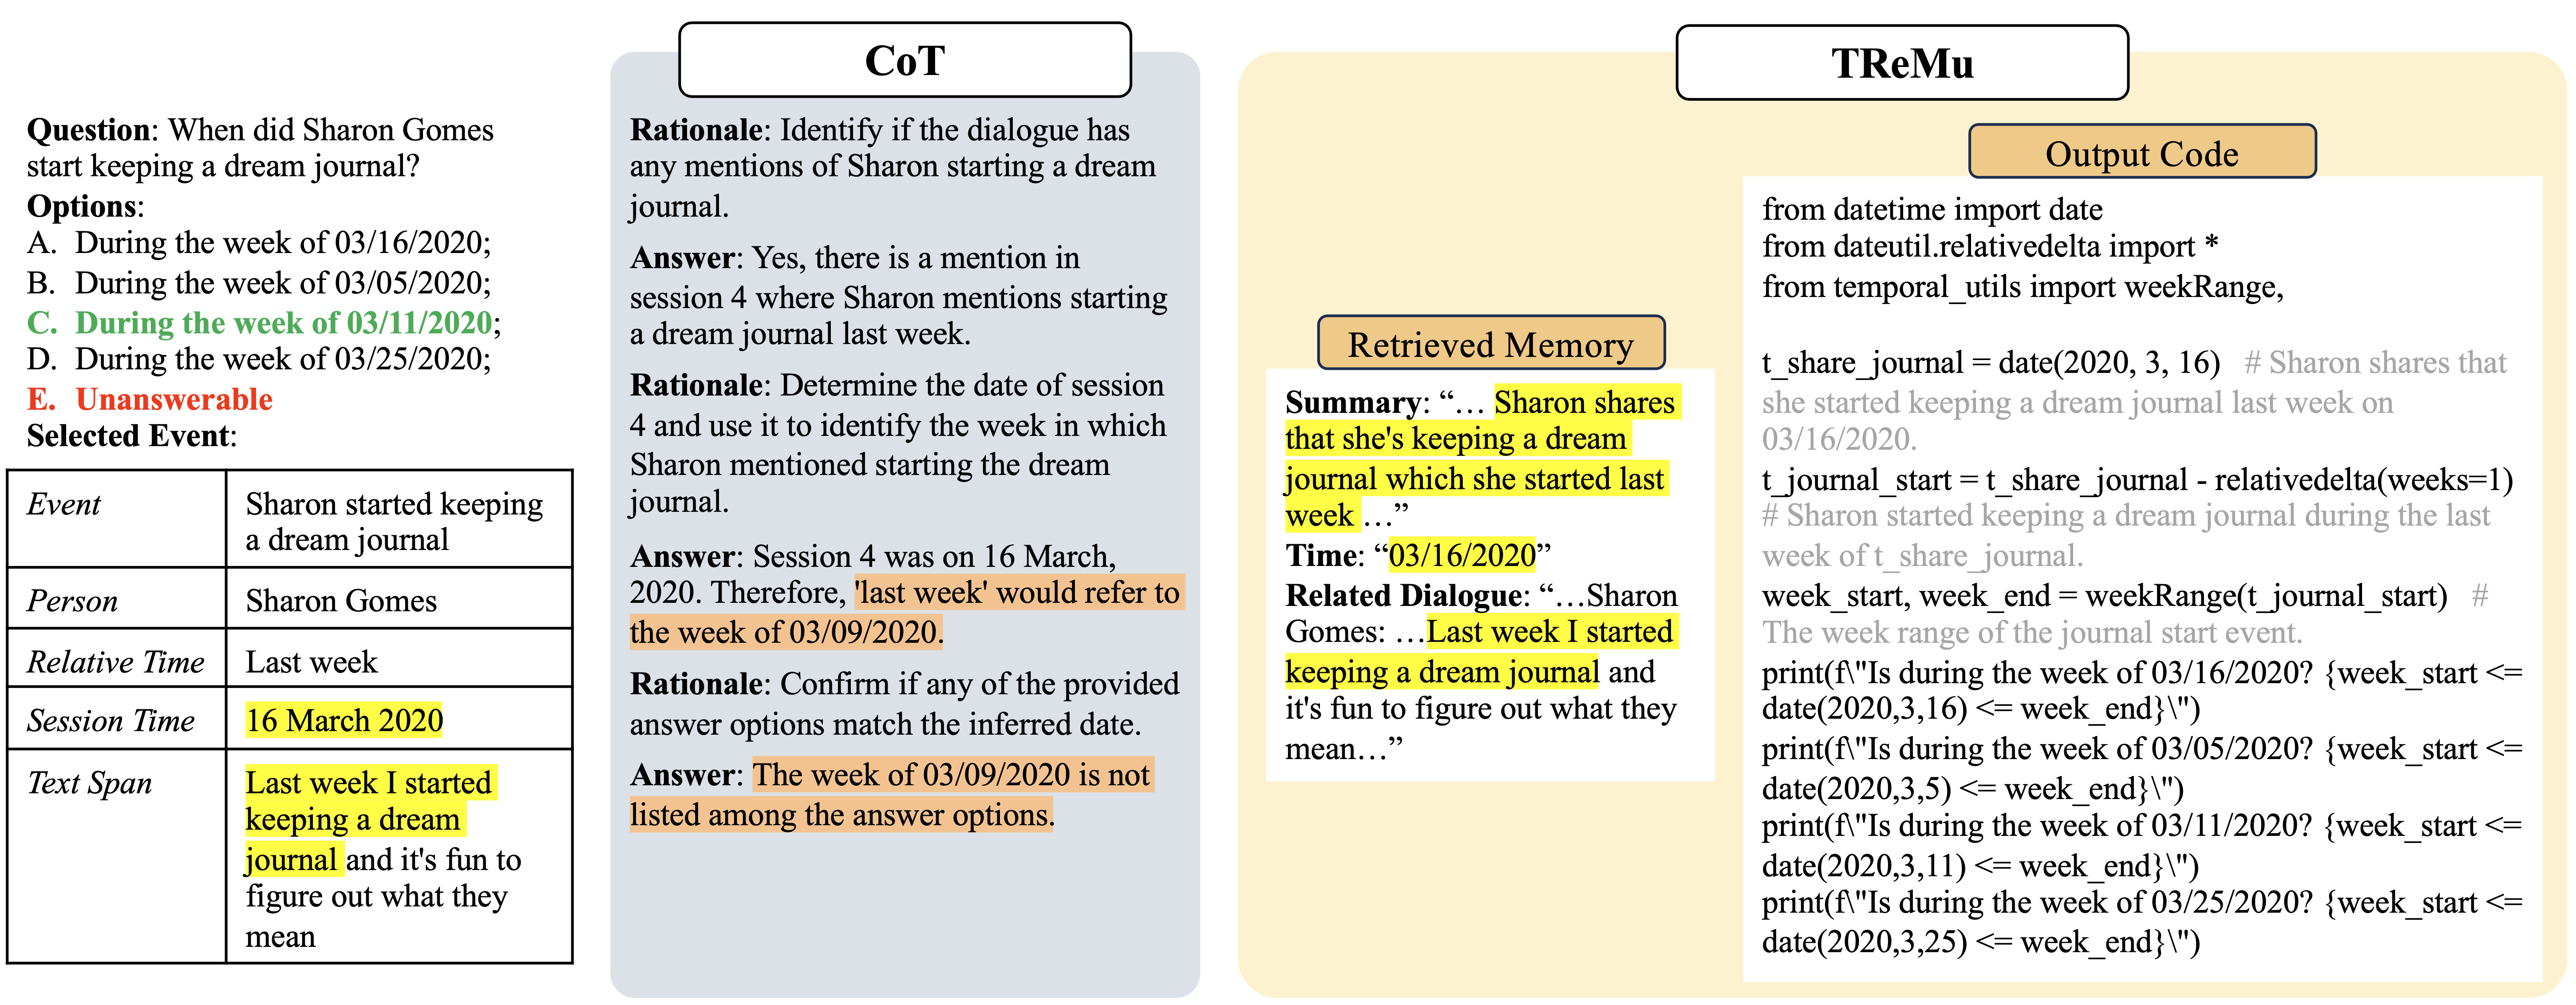
\includegraphics[width=\linewidth]{figures/case_2.png}
    \caption{The second case study comparing CoT and our proposed framework, where CoT results in the wrong answer "E" but our approach selects the correct option "C". We highlight the key information in colors.}
    \label{fig:case_2}
% \vspace{-0.5cm}
\end{figure*}

\subsection{Ablation Study}
From Tables \ref{gpt4o_result}, \ref{gpt4o_mini_result}, and \ref{gpt35_result}, the comparison between MemoChat + CoT and Timeline + CoT highlights the importance of memory representation. Time-aware memorization improves accuracy by instructing models to infer temporal information—particularly relative time—during memorization and mitigate temporal ambiguity. Furthermore, replacing CoT with symbolic reasoning, as seen in the comparison between Timeline + CoT and TReMu, leads to additional performance gains. This improvement stems from the models’ ability to generate Python code while retaining the benefits of step-by-step reasoning. This aligns with recent research integrating LLMs with symbolic reasoners for various reasoning tasks \cite{olausson2023linc,pan2023logic}.

\subsection{Execution Failure Study}
We also measure the percentage of generated code that fails to execute and, during inference, we regenerate the code when such errors occur. The results, shown in Figure \ref{fig:failure}, indicate that the percentages of execution failure are generally low across all three LLMs, demonstrating the reliability of our Python-based symbolic reasoning approach. As expected, GPT-4o exhibits the lowest rate of execution failure, while GPT-3.5-Turbo has the highest, corresponding to the overall performance differences we demonstrate above in temporal reasoning among these models. This likely reflects the inherent performance gap between the LLMs.

\subsection{Case Study}
In this section, we demonstrate how the two key components of our framework—\textit{time-aware memorization} and \textit{neuro-symbolic temporal reasoning}—work in real cases. We compare the outputs of CoT and our framework based on GPT-4o.

In Figure \ref{fig:case_1}, with CoT, even though GPT-4o successfully identifies that the key temporal information is "Sharon's survival course started on 12 March 2020," but it gets confused with "week-long course" and infers the end date of the course, incorrectly selecting "Unanswerable." In contrast, with our framework’s time-aware memorization, the model retrieves the event from memory along with its properly inferred time. During the reasoning stage, the model utilizes this memory to distinguish between when the speaker, Sharon, mentioned the event (03/16/2020) and when the event occurred (03/12/2020). Then the model defines the corresponding variable in the generated code, i.e., \textit{t$\_$start$\_$course}, to precisely capture the time.

Figure \ref{fig:case_2} illustrates another mistake made via CoT. The model correctly infers that the "last week" corresponds to the session time of 16 March 2020 but fails to match the week range with the correct answer—the week of 03/09/2020 is the week of 03/11/2020 but the model does not realize this. As for our framework, the model leverages the Python \textit{dateutil} package's \textit{relativedelta} function, alongside our custom \textit{weekRange} function, to accurately infer the last week's range. This neuro-symbolic reasoning not only facilitates the model to reason step-by-step but also enhances it by incorporating external temporal functions to support more accurate temporal reasoning.